%% Sample essay

\subsection*{Isabelle Goldstick. Path to Individualism (Darwin-Baudelaire)}  
\addcontentsline{toc}{subsection}{Isabelle Goldstick. Path to Individualism (Darwin-Baudelaire)}  

\index{Darwin}
\index{Baudelaire}
\index{Sample essay}

\begin{multicols}{2}
Darwin and Baudelaire. One is a scientist who creates a revolutionary theory, evolution; the other one is a poet who focuses on intensity through his art and his life.
Both look at the past and create the future. Darwin sees evolution leading toward a better humanity, Baudelaire, on the contrary, hates modernity and finds refuge in
intensity. Despite their difference in methods and conclusion, both Darwin's godless universe and Baudelaire's search for pleasure open the door toward individualism.

Darwin’s examination of the past is the key to a new theory explaining the multiplicity of life forms on earth. Rejecting the notion of a divine design and the
idea that life is immutable, he introduces randomness in the life’s creation process. In The Origin of Species, he develops his thoughts on variation and 
natural selection and states that ``Natural Selection \dots\ is as immeasurably superior to man's feeble efforts, as the works of Nature are to those of Art''~[1].
For him, life is the work of nature. The Descent of Man extends natural selection and variation to humans. Men are not created at God’s image or for a great
teleological design, rather “man is descended from some less highly organized form”~[2].

Not surprisingly, Baudelaire approaches these issues quite differently. He is a poet, not a scientist. He observes the world around him and describes it with a mix
of emotion and cynicism, not scientific method. Spleen of Paris describes the Paris of the Second Empire, where poor and rich, dandy and bohemian cross path. In the
poem The Eyes of the Poor, the narrator and his friend are at a cafe and see a poor family. While the narrator is moved and somewhat ashamed, his friend
”can’t stand those people over there, with their eyes wide open like carriage gates!”~[3] and just wants them to disappear. Modernity is disruptive, so will his 
poetry, particularly Spleen of Paris where he finds a way to escape conventions, ignoring
\begin{wrapfigure}{l}{.48\columnwidth}
\copyrightbox[b]{%
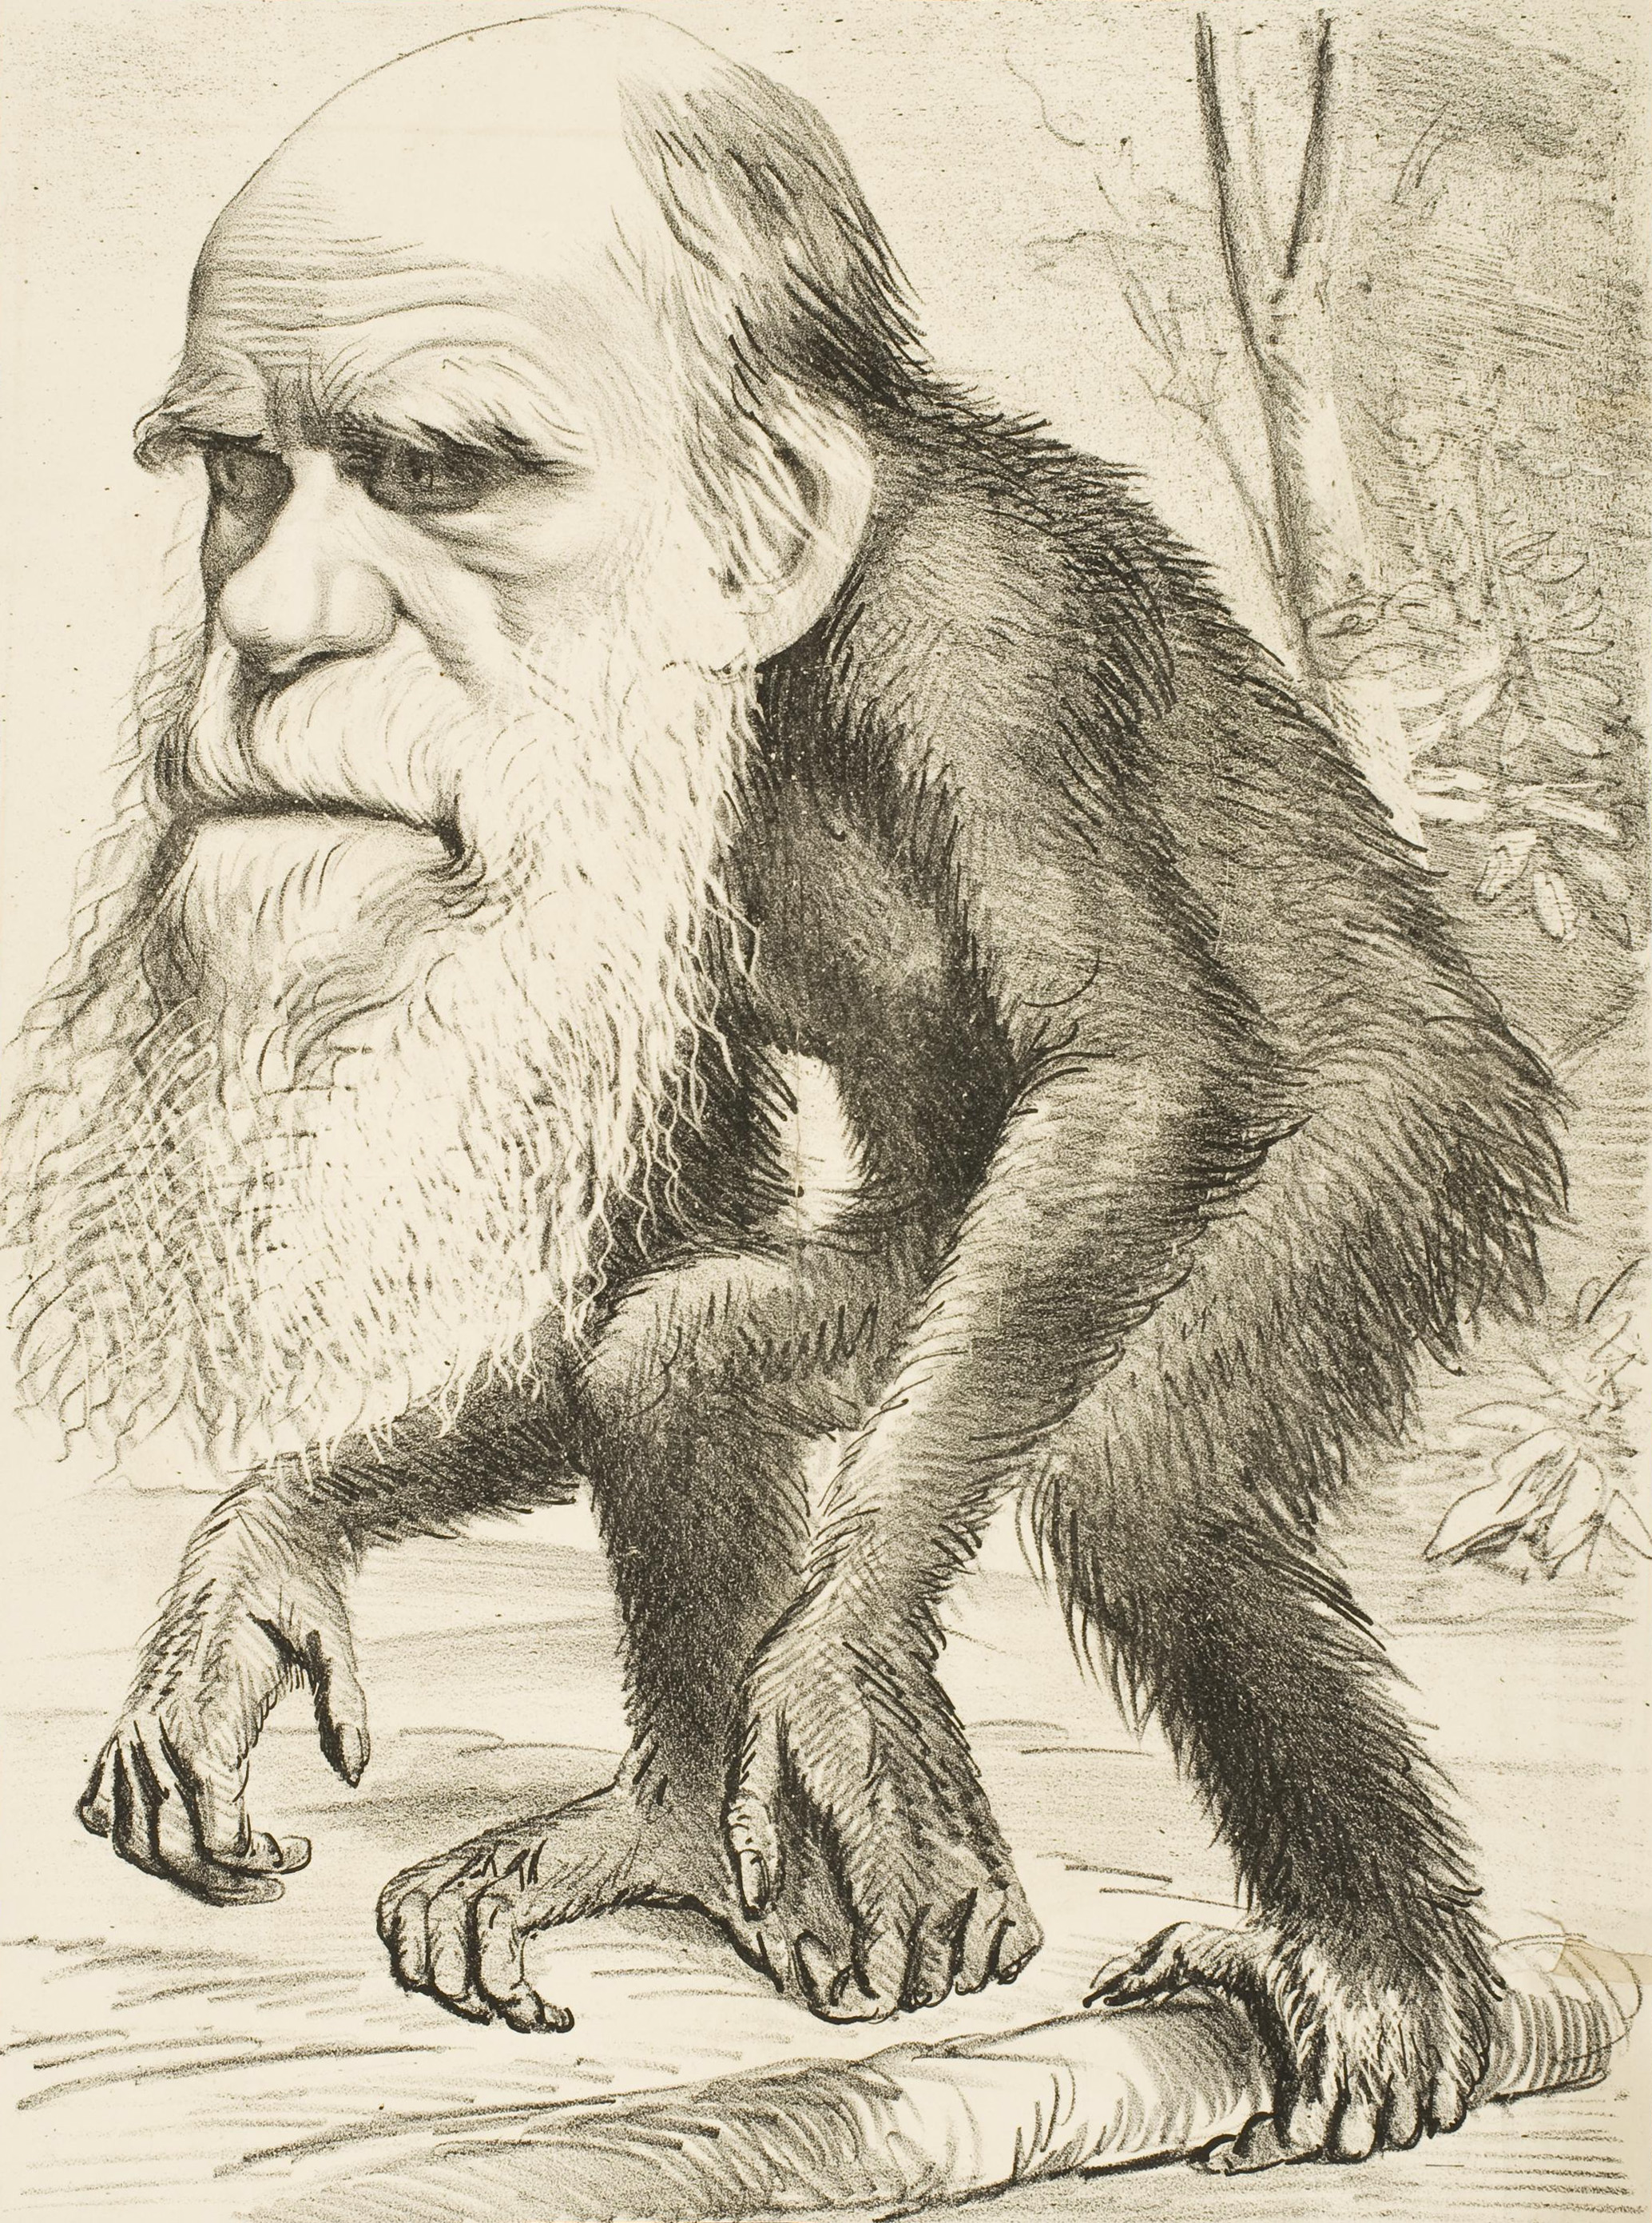
\includegraphics[keepaspectratio,width=.5\columnwidth]{imgs/darwin}}{\centerline{Public Domain}}
\label{img:darwin.jpg}\vspace*{-1.3cm}
\end{wrapfigure}
poetry's rules by writing prose poems. Through these very different lenses,
science and poetry, Darwin and Baudelaire examine the past and reach very different conclusions on the march of humanity.

Darwin uses evolution to examine men as social animals.  Morality, intelligence, language, ``must have been 
all-important to him, \dots, as enabling him to invent
and use language, to make weapons,\dots” and have first be won by natural selection~[2]  As he exposes his ideas on different races and classes, he shows little 
respect for the indigenous populations he meets in his travels, asserting that he would have rather “be descended from that heroic little monkey, \dots\ as from a
savage who delights to torture his enemies,\dots“~[2]. Similarly, he thinks that the very poor are inferior and prevent more affluent and better equipped people from
succeeding. For Darwin, “men still bear the signs of their lowly origins”~[2] though it is clear that some bear it more than others, as his support for the social
order of the Industrial Revolution and colonialism show.   However, humanity progresses positively through education and, in time, it ``may give him hope for a still
higher destiny in the distant future''~[2].

Baudelaire examines the world around him in his Poems in Prose: modernity, bourgeoisie and the class system, all of which are anathema. Let's Beat the Poor is a
good example of this world he despises: the narrator, a bourgeois who has just read modern views on how to fix the world, meets a poor and decides that to be 
“worthy of liberty a man must fight for it”~[3]. This resembles the struggle for life that Darwin describes, but Baudelaire rejects it. Moreover, he sees the
bourgeois way of life as superficial. The bourgeois in A Joker follows conventions slavishly and privileges others' opinion above his own. Baudelaire wants to form
his own mind and rejects this strange world that he feels alienated by: the modern life in the modern metropolis. It is indeed a “strange phenomena we find in a great
city \dots\ Life swarms with innocent monsters.“~[3] It is however unclear who these monsters are, bourgeois, poor or simply, like in To Each His Own Chimera,
modernity. The future is a fatality: people are “driven by an irresistible need to walk” and “are condemned to hope forever”. By comparison, for the poem Evening
Twilight, the past is “delicious” and the present dark.

So, we have a scientist who rejects religion and supports modernity and a poet who, deeply influenced by religion, cannot find solace in it and rejects the modern
world. It is Darwin who changes our view of social values. If morality is not God driven, it is not immutable (men are fallible) and can be adapted to our personal
needs. For Baudelaire, the world is a world of despair, only made worse by his belief in the original sin. He finds no other recourse than the search for intensity
and pleasure, for “\dots\ what is an eternity of damnation compared to an infinity of pleasure in a single second?“~[3]. Individual satisfaction is what matters
whatever the consequences. These authors help us understand how the world will fall into total darkness just a few years later.

\bigskip

\noindent\textbf{\large References}
\begin{enumerate}[{[1]}]
\item Charles Darwin. \textit{The Origins of Species.}
\item Charles Darwin. \textit{The Descent of Man.}
\item Charles Baudelaire. \textit{Spleen of Paris.}
\end{enumerate}
\end{multicols}

